\documentclass[a4paper, 10pt]{article}
\usepackage[utf8]{inputenc} % Change according your file encoding
\usepackage{graphicx}
\usepackage{url}
\usepackage{amsmath}
\usepackage{mathtools}
\usepackage{mathrsfs}
\usepackage{amsfonts}
\usepackage{bbm}
\usepackage{amsthm}
\usepackage{amssymb}
\usepackage{fancyhdr}
\usepackage{setspace}
\usepackage{tabularx}
\usepackage{tikz}
\usetikzlibrary{arrows,positioning}
\usepackage[a4paper, left=2cm, right=2cm, top=2.5cm, bottom=2cm]{geometry}

\pagestyle{fancy}
\fancyhf{}
\rhead{Tuesday, December 10th}
\lhead{Víctor Mart\'in, Pablo Oviedo, and Carlos Segarra - DAG: Sheet 1}
\cfoot{\thepage}

\newtheorem{obs}{Observation}
\newtheorem{theorem}{Theorem}
\newtheorem*{theoremstar}{Theorem}

\theoremstyle{definition} % amsthm only
\newtheorem{definition}{Definition}

%\newtheorem{def}{Definition}

\newcommand{\espai}{\vspace{3mm}}
\newcommand{\I}{\mathscr{I}}
\newcommand{\B}{\mathscr{B}}
\newcommand{\C}{\mathscr{C}}
\newcommand{\F}{\mathscr{F}}

\begin{document}
\onehalfspacing
\tikzstyle{vertice}=[circle, draw, fill=black!50, inner sep = 0pt, minimum width=4pt]

\textbf{\Large Discrete and Algorithmic Geometry: Sheet 1}

\vspace{20pt}

\textbf{\textit{(1) Let $M$ be a matroid on the ground set $[n] = \lbrace 1, 2, \dots, n \rbrace$ with family of independent sets $\lbrace I : I \in \mathcal{I}\rbrace$:}}

\vspace{3pt}

\hspace{5pt} \textbf{\textit{(a) Contracion in $M$ as defined in class agrees with the notion of contraction in graphs.}}

\vspace{3pt}

WRITE HERE

\hspace{5pt} \textbf{\textit{(b) Contracion in $M$ as defined in class agrees with $M / S \coloneqq (M^\star \backslash S)^\star$ for a subset $S \subset [n]$.}}

\vspace{3pt}

WRITE HERE

\vspace{3pt}

\hspace{5pt} \textbf{\textit{(c) $M_{G^\star} = \left(M_G\right)^\star$, if G is a planar graph and $G^\star$ its dual planar graph.}}

%\textbf{\textit{(2) Prove that if a matroid M is realizable over a ground field $\mathbbm{k}$, then the dual matroid $M^\star$ is also realizble over $\mathbbm{k}$.}}

\vspace{3pt}

WRITE HERE

\vspace{3pt}

\hspace{5pt} \textbf{\textit{(d) Consider the matroid M realized by the columns of the matrix}}
$$
A = \left[
    \begin{array}{ccccc}
        0 & 1 & 1 & 0 & 1 \\
        1 & 0 & 1 & 0 & 1 \\
        0 & 1 & 1 & 1 & 0
    \end{array}
\right]
$$
\textbf{\textit{Compute a realization of $M^\star$, and some contractions of M of your choosing. Compute the set of circuits and cocircuits of $M$ and of $M^\star$.}}

\vspace{5pt}

We will first compute a realization of matrix A.
To do so, we will swap columns two and four and perform a change of basis to basis $\mathcal{B} = \left\lbrace \left( \begin{array}{c} 0 \\ 1 \\ 0 \end{array} \right), \left( \begin{array}{c} 1 \\ 0 \\ 1 \end{array} \right), \left( \begin{array}{c} 1 \\ 1 \\ 1 \end{array} \right) \right\rbrace$. We then have,
\begin{equation*}
    \begin{split}
        A & = \left[
            \begin{array}{ccccc}
                0 & 1 & 1 & 0 & 1 \\
                1 & 0 & 1 & 0 & 1 \\
                0 & 1 & 1 & 1 & 0
            \end{array}
        \right]
        \longrightarrow
        \left[
            \begin{array}{ccccc}
                0 & 0 & 1 & 1 & 1 \\
                1 & 0 & 1 & 0 & 1 \\
                0 & 1 & 1 & 1 & 0
            \end{array}
        \right]
        \overset{\mathcal{B}}{\longrightarrow}
        \bar{A} = \left[
            \begin{array}{ccccc}
                1 & 0 & 0 & -1 & 0 \\
                0 & 1 & 0 & 0 & -1 \\
                0 & 0 & 1 & 1 & 1
            \end{array}
        \right]
        \hspace{10pt} \text{ which also represents $M$.} \\[10pt]
        \bar{A}B^T & = 0 \Longrightarrow 
        B^T = \left[
            \begin{array}{cc}
                -1 & 0  \\
                0  & -1 \\
                1  & 1 \\
                -1 & 0 \\
                0 & -1
            \end{array}
        \right] \hspace{5pt} \text{ (for example) } \Longrightarrow
        B = \left[
            \begin{array}{ccccc}
                -1 & 0 & 1 & -1 & 0 \\
                0 & -1 & 1 & 0 & -1
            \end{array} 
        \right] \hspace{5pt} \text{ which is $M^*$.}
    \end{split}
\end{equation*}

Now we will compute a contraction of $M$, $M / 1$, using a deletion in its dual matroid, $M^*$, $(M^* \backslash 1)^*$.
\begin{equation*}
    \begin{split}
        B \backslash 1 & = \left[
            \begin{array}{cccc}
                0 & 1 & -1 & 0 \\
                -1 & 1 & 0 & -1 
            \end{array} 
        \right] \text{ ;} \hspace{5pt}
        (B  \backslash 1)\cdot c^T = 0 \Rightarrow 
        c^T = \left[
                \begin{array}{cc}
                    0 & 1 \\
                    1 & 1 \\
                    1 & 1 \\
                    1 & 0
                \end{array} 
            \right] \Rightarrow
        c = \left[
                \begin{array}{cccc}
                    0 & 1 & 1 & 1 \\
                    1 & 1 & 1 & 0
                \end{array} 
            \right] \hspace{3pt} \text{which is $M / 1$.}
    \end{split}
\end{equation*}

An alternative method for computing $ M / 1$ is doing the projection in the corresponding direction. In particular, to find $ M / 1$ it suffices to project $A$ in direction $\left( \begin{array}{ccc} 0 & 1 & 0 \end{array} \right)^T$ and get rid of loops. In particular,
\begin{equation*}
    \begin{split}
        A & = \left[
            \begin{array}{ccccc}
                0 & 0 & 1 & 1 & 1 \\
                1 & 0 & 1 & 0 & 1 \\
                0 & 1 & 1 & 1 & 0
            \end{array}
        \right]
        \overset{\text{\footnotesize{Project}}}{\longrightarrow}
        \left[
            \begin{array}{ccccc}
                0 & 0 & 1 & 1 & 1 \\
                0 & 1 & 1 & 1 & 0
            \end{array}
        \right]
        \overset{\text{\footnotesize{No Loops}}}{\longrightarrow}
        \left[
            \begin{array}{ccccc}
                0 & 1 & 1 & 1 \\
                1 & 1 & 1 & 0
            \end{array}
        \right] \hspace{5pt} \text{ which again is $ M / 1$.}
    \end{split}
\end{equation*}

Lastly, circuits are minimal linear combinations, and co-circuits are their dual counterparts.
Hence, computing both the circuits of $M$ and $M^*$ we will also have the co-circuits of $M^*$ and $M$ respectively.
In particular, by inspection we have:
\begin{equation*}
    \text{Circuits of $M$ } = (-1, 0, 1, -1, 0), (0, -1, 1, 0, -1) = \text{ Cocircuits of $M^*$}
\end{equation*}
\begin{equation*}
    \text{Circuits of $M^*$ } = (1, 1, 1, 0, 0), (0, 0, 1, 1, 1), (1, 0, 0, -1, 0), (0, 1, 0, 0, -1) = \text{ Cocircuits of $M$}
\end{equation*}


\vspace{5pt}

\begin{center}
    \rule{5cm}{0.4pt}
\end{center}

\newpage

\textbf{\textit{(2) Let $A \in \mathbb{R}^{n\times d}$ be a matrix of full rank, and let the columns of $B \in \mathbb{R}^{n \times (n -d)}$ be a basis of the row space of $A$, so that $AB = 0$ and the rows of $B$ are a Gale transform of the columns of $A$. We saw in class that $\text{LinVal}(A) = \text{LinDep}(B)$. Show that $\text{LinVal}(B) = \text{LinDep}(A)$.}}

\vspace{3pt}

WRITE HERE


\vspace{5pt}

\begin{center}
    \rule{5cm}{0.4pt}
\end{center}

\newpage

\textbf{\textit{(3) The greedy algorithm always works for matroids.}}

\hspace{5pt}\textbf{\textit{(a) Show that Kruskal's greedy algorithm always finds a maximum weight independent set in a matroid $M = (E, \mathcal{I})$, regardless of the choice of weight function $\omega : E \mapsto \mathbb{R}_{>0}$. Recall that the greedy algorithm starts by setting $I \coloneqq \emptyset$, and next repeatedly chooses $y \in E \backslash I$ with $I \cup \lbrace y \rbrace \in \mathcal{I}$ and with $\omega(y)$ as large as possible. It stops if no such $y$ exists.}}

\vspace{3pt}

Let us rename the independent sets $I_0, I_1, \ldots, I_r$, where $I_0 = \emptyset$, and $I_{j+1} = I_j \cup \{y_j\}$, for some $y_j \in E \setminus I_j$ with $\omega y_j$ as large as possible. Let us show $|I_j| = j$ by induction, and that, assuming $E$ is finite, there exists a final $I_r$, for some $r$ that satisfies $r = \max_{I \in \mathcal I} |I|$.

For $j = 0$, $|I_0| = |\emptyset| = 0$
For $j > 0$, assuming induction hypothesis, $I_{j+1} = I_j \cup \{y_j\}$, for some $y_j \in E \setminus I_j$, and therefore $|I_{j+1}| = |I_j| + 1 = j + 1$. Assume that the last independendent set is $I_s$ for some $s$. Obviously, $s \leq r = \max_{I \in \mathcal I} |I|$, since $I_s \in \mathcal I$. If $s < r$, there will be a set $I'$ with $|I'| = r$. By the exchange axiom, there would be an $y_s \in I' \setminus I_s \subset E \setminus I_s$ such that $I_s \cup \{y_s\} \in \mathcal I$, leading to a contradiction since $|I_s \cup \{y_s\} \in \mathcal I| = s + 1 > s$.

We are left with proving that the weight we obtain with the algorithm is indeed the maximum achievable. Let us show by induction that $I_j$ is contained in an optimal basis $B$.

For the case $j = 0$, it is trivial, since $\emptyset = I_0 \subset B$. Now, applying induction hypothesis, if $I_j \subset B$, let us see what happens for $I_{j+1} = I_j \cup \{y_j\}$. If $y_j \in B$, $I_{j+1} \subset B$, so let us assume $y_j \notin B$. In this case $I_{j+1} \not\subset B$, but $I_{j+1} \subset B'$ for some basis $B'$ which is not optimal. By the exchange axiom, since $y_j \in B' \setminus B$, there is $y_j' \in B \setminus B'$ such that $B'' = B \setminus \{y_j'\} \cup \{y_j\}$ is a basis. $I_j \cup \{y_j'\}$ is independent as well since it is contained in a basis. By the construction of the algorithm, $\omega(y_j') \leq \omega(y_j)$. This implies that
\[
\sum_{b \in B} \omega(b) =
w(y_j') + \sum_{b \in B, b \neq y_j'} \omega(b) \leq
w(y_j) + \sum_{b \in B, b \neq y_j} \omega(b) =
\sum_{b \in B \setminus \{y_j'\} \cup \{y_j'\}} \omega(b) =
\sum_{b \in B''} \omega(b),
\]
Meaning that $B''$ is another optimal basis that contains $I_{j+1}$.

Finally, $I_r$, since its size will be the maximum set of an independent set, and therefore is a basis. Since a basis cannot be contained in another basis, $I_r$ will be the optimal basis.
\vspace{3pt}

\hspace{5pt}\textbf{\textit{(b) Show that that this property characterizes independent sets of matroids among all simplicial complexes. In other words, given a simplicial complex $\Sigma$ for which the greedy algorithm always works, regardless of the weight function~$\omega$, show that $\Sigma = \mathcal I(M)$ for some matroid~$M$.}}

\vspace{3pt}

WRITE HERE


\vspace{5pt}

\begin{center}
    \rule{5cm}{0.4pt}
\end{center}

\newpage

\textbf{\textit{(4) Using a famous result by Jack Edmonds, prove the following:}}

\hspace{5pt}\textbf{\textit{(a) Let $G=(V,E)$ be a bipartite graph with color classes $V_1,V_2$. For $i=1,2$, let $M_i$~be the matroid where $I\subseteq E$ is independent if and only if each vertex in~$V_i$ is covered by at most one edge in~$I$. Use the Matroid Intersection Theorem to prove:}}
    \begin{theoremstar}[K\H onig's Matching Theorem]
      The maximum size of a matching in a bipartite graph equals the minimum size of a vertex cover.
    \end{theoremstar}

\vspace{3pt}

WRITE HERE

\vspace{3pt}

\hspace{5pt}\textbf{\textit{(b) Let $G=(V,E)$ be a graph whose edges are partitioned into $k$~colors, $E=E_1\cup E_2\cup\cdots\cup E_k$. Use the Matroid Intersection Theorem to prove that there exists a rainbow spanning tree (a spanning tree all of whose edges are colored differently) if and only if $G-F$ has at most $t+1$ connected components, for any union~$F$ of $t$~colors, for any $t\ge0$.}}

\vspace{3pt}

WRITE HERE


\vspace{5pt}

\begin{center}
    \rule{5cm}{0.4pt}
\end{center}

\newpage

\textbf{\textit{(5) Let $\cT=\{\sigma_1,\dots,\sigma_m\}$ be a triangulation of a full-dimensional point configuration $\cA=(\aaa_1,\dots,\aaa_n)\subset\RR^d$ of $n$~points, where we consider the $\sigma_i\in\binom{[n]}{d+1}$ to be index sets. Let $R^{\text{int}}$ be the set of interior ridges, defined to be intersections $\rho = \rho_{ij} = \sigma_i\cap\sigma_j$ of two facets of~$\cT$ such that the affine span of the points of~$\cA$ indexed by~$\rho$ has dimension~$d-1$. (In the triangulations of~Figure~\ref{fig:triangs1}, they are the interior edges.)}}

  \begin{figure}[htbp]
    \centering
    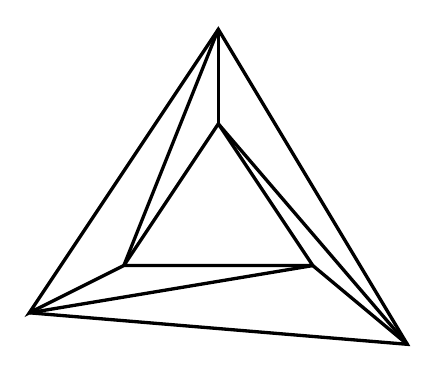
\begin{tikzpicture}[scale=.4]
      \coordinate (1) at (0,0);
      \coordinate (2) at (12,-1);
      \coordinate (3) at (6,9);
      \coordinate (4) at (3,1.5);
      \coordinate (5) at (9,1.5);
      \coordinate (6) at (6,6);

      \draw[very thick] (1)--(2)--(3)--(1)--(4)--(5)--(6)--(4);
      \draw[very thick] (2)--(5);
      \draw[very thick] (3)--(6);

      \draw[very thick] (1)--(5);
      \draw[very thick] (2)--(6);
      \draw[very thick] (3)--(4);
    \end{tikzpicture}
    \qquad
    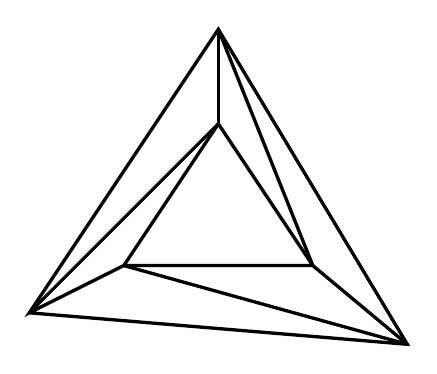
\begin{tikzpicture}[scale=.4]
      \coordinate (1) at (0,0);
      \coordinate (2) at (12,-1);
      \coordinate (3) at (6,9);
      \coordinate (4) at (3,1.5);
      \coordinate (5) at (9,1.5);
      \coordinate (6) at (6,6);

      \draw[very thick] (1)--(2)--(3)--(1)--(4)--(5)--(6)--(4);
      \draw[very thick] (2)--(5);
      \draw[very thick] (3)--(6);

      \draw[very thick] (2)--(4);
      \draw[very thick] (3)--(5);
      \draw[very thick] (1)--(6);
    \end{tikzpicture}    
    \caption{Two triangulations.
    View the source code for the coordinates of the points.}
    \label{fig:triangs1}
  \end{figure}

\begin{enumerate}
  \item
    For a vector $\omega\in\RR^n$, lift the points in $\cA$ to heights~$\omega$, so that
    $\cA^\omega=\big(\binom{\aaa_1}{\omega_1},\dots,\binom{\aaa_n}{\omega_n}\big)$.
    For each interior ridge $\rho=\sigma_i\cap\sigma_j\in R^{\text{int}}$,
    formulate the folding condition that expresses that $\rho$ indexes a face of the lower convex hull of~$\cA^\omega$,
    in terms of the coordinates of the~$\aaa_i$ and~$\omega$.
    Your folding condition should be an inequality that is linear in each height~$\omega_i$.

To formulate the folding condition, we make use of Definition 7.4 in Rheka R. Thomas~\footnote{Rekha R. Thomas. Lectures in geometric combinatorics., volume 33 of Student Mathematical Library. Providence, RI: American Mathematical Society (AMS); Princeton, NJ: Institute for Advanced Studies, 2006.}:
        \begin{equation*}
            bla
        \end{equation*}

  \item
    Write code that takes the coordinates of the $\aaa_i$ and the facets $\sigma_i$ of a triangulation as input,
    and outputs the set of folding conditions in a text file in
    LP file format.

  \item
    Download a linear programming software such as
    \texttt{gurobi},
    \texttt{cplex} or
    \texttt{scip}/\texttt{soplex}
    and check explicitly whether there exists a choice of heights $\omega$ that induces each of the triangulations of Figure~\ref{fig:triangs1}.

  \item
    Using this code,
    check that the triangulation of the $4$-dimensional cube from~\cite{deLoera96}
    given by the files \texttt{4-cube.vertices} and \texttt{4-cube.triangulation}
    is non-regular, i.e., it does not come from a lifting to~$\RR^5$.
    If you like, download and play with TOPCOM.
  \end{enumerate}


\vspace{5pt}

\begin{center}
    \rule{5cm}{0.4pt}
\end{center}

\newpage

\textbf{\textit{(7) In each of the classes or models of matroids discussed in class (linear / graphical / transversal / algebraic matroids; hyperplane / affine hyperplane arrangements, matroid polytopes),}}

\hspace{5pt}\textbf{\textit{(a) describe independent sets, bases, circuits, cocircuits, and flats.}}

\vspace{3pt}

\begin{table}[]
\begin{tabular}{lllll}
                 & Linear                                                                                                                                     & Graphical                                 & Transversal       & Algebraic                                                                                                                         \\
Independent sets & Sets of linearly independent vectors                                                                                                       & Sets of edges that do not form any cycles & Matchings         & Sets of elements $\{\alpha_i\}$ that are algebraically independent and such that $\mathbb K[\{\alpha_i\}] \subset L$ is algebraic \\
Bases            & Bases (in the linear algebra sense)                                                                                                        & Spanning trees of a graph                 & Maximal matchings & Sets of elements $\{\alpha_i\}$ that are algebraically independent and such that $\mathbb K[\{\alpha_i\}] = L$                    \\
Circuits         & Sets ${v_1, \ldots, v_k\}$ such that $a_1 v_1 + \ldots + a_k v_k = 0$ for unique (up to multiplicative constant) $a_1, \ldots, a_k \neq 0$ (or, equivalent, such that no $k-1$ vectors out of the $k$ ones are on the same $k-2$-dimensional space & Simple cycles                             &                   &                                                                                                                                   \\
Cocircuits       &                                                                                                                                            &                                           &                   &                                                                                                                                   \\
Flats            & Sets of vector that generate all the vector space                                                                                          & Connected graphs                          & Maximal matchings & Sets of elements $\{\alpha_i\}$ such that $\mathbb K[\{\alpha_i\}] = L$                                                          
\end{tabular}
\end{table}
\vspace{3pt}

\hspace{5pt}\textbf{\textit{(b) For which of these entities can you rapidly see that they fulfill the corresponding axiom systems?  For which does it seem mysterious?.}}

\vspace{3pt}

WRITE HERE

\vspace{3pt}

\hspace{5pt}\textbf{\textit{(c) Describe the dual matroid of a matroid in each of these situations.}}

\vspace{3pt}

WRITE HERE


\vspace{5pt}

\begin{center}
    \rule{5cm}{0.4pt}
\end{center}

\newpage

\textbf{\textit{(8) We have seen that a matroid can be given by its collections of independent sets, bases, circuits, cocircuits, flats, or its rank function. Find algroithms to convert between as many of these entitites as you can. What is their combinatorial complexity?}}

\vspace{3pt}

For the rest of the exercise, it will be useful having the following graph in mind.
We will refer to specific algorithms by the letter of their edge.
In doing so, we won't assume anything on our ground set, neither on a theoretical implementation, we will just focus on the combinatorial complexity.
Note that we have chosen this \textit{bipartite} representation to improve readability.

\begin{center}
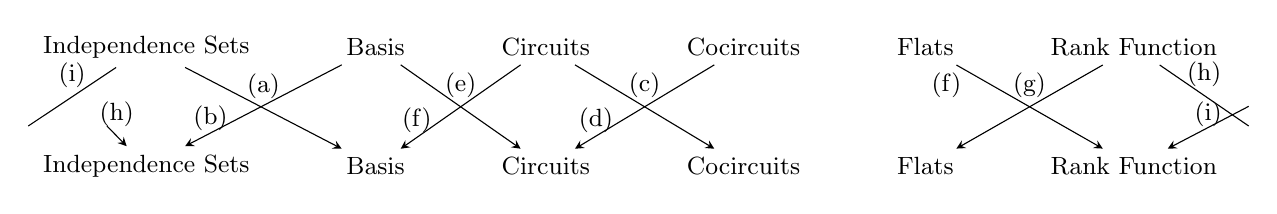
\begin{tikzpicture}\small
  \tikzset{>=stealth}
    % Top Row Nodes
    \node (independence-sets) {Independence Sets};
    \node [right=of independence-sets] (basis) {Basis};
    \node [right=of basis] (circuits) {Circuits};
    \node [right=of circuits] (cocircuits) {Cocircuits};
    \node [right=of cocircuits] (flats) {Flats};
    \node [right=of flats] (rank) {Rank Function};
    % Bottom Row Nodes
    \node [below=of independence-sets] (independence-sets-b) {Independence Sets};
    \node [right=of independence-sets-b] (basis-b) {Basis};
    \node [right=of basis-b] (circuits-b) {Circuits};
    \node [right=of circuits-b] (cocircuits-b) {Cocircuits};
    \node [right=of cocircuits-b] (flats-b) {Flats};
    \node [right=of flats-b] (rank-b) {Rank Function};
    \draw[->] (independence-sets) --  (basis-b) node[midway, above] {(a)};
    \draw[->] (basis) -- (independence-sets-b) node[near end, above, xshift = -5pt, yshift = -5pt] {(b)};
    \draw[->] (circuits) --  (cocircuits-b) node[midway, above] {(c)};
    \draw[->] (cocircuits) -- (circuits-b) node[near end, above, xshift = -5pt, yshift = -5pt] {(d)};
    \draw[->] (basis) --  (circuits-b) node[midway, above] {(e)};
    \draw[->] (circuits) -- (basis-b) node[near end, above, xshift = -5pt, yshift = -5pt] {(f)};
    \draw[->] (rank) --  (flats-b) node[midway, above] {(g)};
    \draw[-] (rank) --  (14,-1) node[midway, above] {(h)};
    \draw[->] (-0.5,-1) --  (independence-sets-b) node[midway, above] {(h)};
    \draw[-] (independence-sets) --  (-1.5,-1) node[midway, above] {(i)};
    \draw[->] (14,-0.75) --  (rank-b) node[midway, above, yshift=-3pt] {(i)};
    \draw[->] (flats) --  (rank-b) node[midway, above, xshift=-30pt, yshift=-0pt] {(f)};
  \end{tikzpicture}
\end{center}

Beneath we describe each algorithm indexed by the label of the edge and include its complexity:
\begin{itemize}
    \item[(a)] 
        We have that a set is independent if and only if it is a subset of a basis.
        In other words, a basis is a maximaly independent set.
        To obtain $\B$ from $\I$ we iteratively, add independent elements to our basis with the caveat that subsets of already existing elements are discarded, and elements containing an already included one are swapped.
        The combinatorial complexity is $\mathcal{O}(|\I|^2)$.
    \item[(b)] Symetrically, $\I$ is the power set of $\B$, from which the algorithm clearly follows. The complexity is ruled by printing or returning all elements in the set, which is $\mathcal{O}\left(\mathcal{P}(|\B|)\right)$.
    \item[(c)] Hull, B. \footnote{Hull, B. \textit{Two algorithms for Matroids}. Discrete Mathematics, Volume 13, Issue 2, 1975, Pages 121-128} presents an algorithm to, given the circuits of a matroid, find those of its dual matroid. The algorithm builds an element from $\C^*$ starting from one in $\C$ and using the elements of $E$. The algorithm in detail uses a recursion for which a more precise complexity calculation would be required. It is clear that, if we have the circuits of the dual matroid, we can find the cocircuits of the original one in linear time.
    \item[(d)] As proven in class, finding the dual of a matroid is linear in its size (doing Gauss). Further, given that the cocricuits are the circuits of the dual matroid, to obtain the cocircuits we can find the dual of the matroid (lineal time) and then apply (c).
    \item[(e)] A circuit is a minimally dependent set, all its proper subsets are independent. If we are given $\B$, we have to check whether adding a new element of $E$ creates a circuit or not. Note that, $\forall x \in E, \B \cup x$ contains one circuit but we want to make sure that it is minimally dependent. The algorithm consists then in for each $B \in \B = {x_1, \dots, x_b}$ and for each $x \in E$ we generate a circuit $C$ consisting of $x \cup \lbrace x_i : x_i \in B \wedge B \cup \{ x\} - x_i \in \B \rbrace$. The algorithm's complexity is then $\mathcal{O}\left(|\B||E||B|\right)$\footnote{E. Minieka, \textit{Finding the Circuits of a Matroid}. Journal of research of the National Bureau of Standards.}.
    \item[(f)] To obtain the basis of a matroid from its circuits, we have found a very intuitive and graphical algorithm presented by Hull in $1975^1$. In essence, it uses that no subset of a circuit is a circuit, and hence looks for a unique element in each circuit (it must exist) that makes it be minimally dependent. Removing it turns that circuit into a base. Looking for this odd elements (called \textit{pegs} in the original algorithm) can be done in linear time if implemented correctly. Then to find all basis we need to find all orderings of the induced basis from circuits. This last step rules our complexity.
    \item[(g)] This algorithm stems from the definition of a flat. A flat is a set whose closure is equal to itself, it is maximal in its rank. This is, adding an element would increase it's size. A naive algorithm would then be: for each subset  $S \subset E$, test the rank of $S \cup \{x \}$ for all $x \in E$ not in $S$. If every one adds to the current rank of $S$, then $S$ is a flat. The algorithm has complexity $\mathcal{O}(\mathcal{P}(E) \cdot |E|)$.
    \item[(h)] This algorithm also stems immediately from the fact that $A \subset E$ is an independence set iff it's rank equals its cardinality.
    \item[(i)] The rank function of a matroid, maps sets of elements to their rank. If a set $S \subset E$ belongs to $\I$, then it's rank will be its cardinality. Otherwise, the rank is the size of the maximum independence subset in $S$. A naive algorithm could be the following: for all $S \in E$, if $S \in \I$ we return $|S|$, otherwise, for each $U \in \I$ we look for that of maximum cardinality which is a subset of $S$. Hence, we can determine the rank of a set in $\mathcal{O}(|\I|)$.
    \item[(j)] We can implement a black-box style rank function using only the set of flats. To do so, we need to first know the maximum rank, $R$, of the sets of flats, $\F$. Then, given $S \subset E$, if $|S| = |E|$ we have its rank, which is maximum. Otherwise, we look for an element $F \in \F$ with only one element more, and compute the number of steps we take until we reach $E$. This number is the corank, which yields the corank. Alternatively, we could build the lattice of flats and compute this height manually.  
\end{itemize}

As a disclaimer and to finalize the exercise, we would like to note that we only present a subset of the algorithms we found.
Given the inherent (by definition) equivalences among many of the collections we defined, most algorithms could be easily rephrased to start from a different collection.
We have provided the sufficient selection to, concatenating one with the other, be able to get from any starting point to any ending point.


\vspace{5pt}

\begin{center}
    \rule{5cm}{0.4pt}
\end{center}

\end{document}
